\section{问题一模型的建立与求解}

\subsection{模型建立}

问题一给定典型日风光出力曲线和常规负荷曲线，电解槽与合成氨装置满负荷连续运行（36吨/日，20.75 MW），不计功率损耗。这是一个确定性的功率平衡核算问题，通过解析计算即可得到各时段的购售电功率及全日累计指标。

\textbf{第一步：功率平衡。}园区内部所有发电功率与用电功率必须实时平衡。以小时为时段单位，$t=0,\ldots,23$。发电侧包括风电$P_{\mathrm{w}}(t)$、光伏$P_{\mathrm{pv}}(t)$和网购电力$P_{\mathrm{b}}(t)$；用电侧包括常规负荷$P_{\mathrm{L}}(t)$、制氢氨负荷$P_{\mathrm{prod}}(t)$和售电$P_{\mathrm{s}}(t)$。功率平衡方程为：
\begin{equation}
P_{\mathrm{w}}(t) + P_{\mathrm{pv}}(t) + P_{\mathrm{b}}(t) = P_{\mathrm{L}}(t) + P_{\mathrm{prod}}(t) + P_{\mathrm{s}}(t) \label{eq:q1_balance}
\end{equation}

各功率分量由附件给出的标幺值乘以对应装机容量计算得到。风电装机40 MW、光伏装机64 MW、常规负荷峰值6 MW，制氢氨在满发条件下恒为20.75 MW：
\begin{align}
P_{\mathrm{w}}(t) &= 40 \times \text{风电标幺值}(t),\; P_{\mathrm{pv}}(t) = 64 \times \text{光伏标幺值}(t) \notag \\
P_{\mathrm{L}}(t) &= 6 \times \text{负荷标幺值}(t),\; P_{\mathrm{prod}}(t) \equiv 20.75 \notag
\end{align}

购电和售电在任一时段不能同时发生，因此需要根据供需差额判定。引入净负荷$N(t)$表示风光出力减去常规负荷和制氢氨负荷后的剩余：
\begin{equation}
N(t) = P_{\mathrm{w}}(t) + P_{\mathrm{pv}}(t) - P_{\mathrm{L}}(t) - P_{\mathrm{prod}}(t) \label{eq:q1_net}
\end{equation}
当$N(t) \ge 0$时，风光出力有盈余，余电上网$P_{\mathrm{s}}(t)=N(t)$；当$N(t) < 0$时，出力不足，需网购电力$P_{\mathrm{b}}(t) = -N(t)$：
\begin{equation}
P_{\mathrm{s}}(t) = \max\{N(t), 0\},\quad P_{\mathrm{b}}(t) = \max\{-N(t), 0\} \label{eq:q1_bs}
\end{equation}

\textbf{第二步：全日累计电量。}计算出各时段购售电功率后，需汇总全日总量以计算绿电指标。全日新能源发电量$E_{\mathrm{re}}$、总用电量$E_{\mathrm{total}}$、上网电量$E_{\mathrm{sell}}$和网购电量$E_{\mathrm{buy}}$分别为各时段对应功率的累加：
\begin{align}
E_{\mathrm{re}} &= \sum_{t=0}^{23} [P_{\mathrm{w}}(t) + P_{\mathrm{pv}}(t)] \label{eq:q1_ere} \\
E_{\mathrm{total}} &= \sum_{t=0}^{23} [P_{\mathrm{L}}(t) + P_{\mathrm{prod}}(t)] \label{eq:q1_etotal} \\
E_{\mathrm{sell}} &= \sum_{t=0}^{23} P_{\mathrm{s}}(t),\quad E_{\mathrm{buy}} = \sum_{t=0}^{23} P_{\mathrm{b}}(t) \label{eq:q1_ebs}
\end{align}

\textbf{第三步：绿电直连指标。}根据国家绿电直连项目要求，需考核以下三项指标。自发自用比例$R_{\mathrm{sc}}$衡量新能源发电量中园区自用的比例，总用电绿电比例$R_{\mathrm{g}}$衡量用电量中绿电的占比，上网电量比例$R_{\mathrm{cur}}$衡量新能源发电量中上网的比例：
\begin{align}
R_{\mathrm{sc}} &= \frac{E_{\mathrm{total}} - E_{\mathrm{sell}} - E_{\mathrm{buy}}}{E_{\mathrm{re}}} \ge 60\% \label{eq:q1_sc} \\
R_{\mathrm{g}} &= \frac{E_{\mathrm{re}} - E_{\mathrm{sell}}}{E_{\mathrm{total}}} \ge 30\% \label{eq:q1_gr} \\
R_{\mathrm{cur}} &= \frac{E_{\mathrm{sell}}}{E_{\mathrm{re}}} \le 20\% \label{eq:q1_cur}
\end{align}

\textbf{第四步：吨氨成本。}吨氨成本是评价园区经济效益的核心指标，由发电成本、购售电净成本和运维成本三部分构成：
\begin{equation}
C_{\mathrm{NH_3}} = \frac{C_{\mathrm{gen}} + C_{\mathrm{grid}} + C_{\mathrm{OM}}}{Q_{\mathrm{NH_3}}} \label{eq:q1_cost}
\end{equation}
其中发电成本按风电度电成本0.15元/kWh和光伏度电成本0.12元/kWh计算，购售电净成本反映园区与电网交易的结果（正为净支出、负为净收入），运维成本按设备运行时间线性计算：
\begin{align}
C_{\mathrm{gen}} &= \sum_{t=0}^{23} [P_{\mathrm{w}}(t) \times 150 + P_{\mathrm{pv}}(t) \times 120] \quad [\text{元}] \\
C_{\mathrm{grid}} &= \sum_{t=0}^{23} [P_{\mathrm{b}}(t)C_{\mathrm{b}}(t) - P_{\mathrm{s}}(t)C_{\mathrm{s}}] \quad [\text{元}] \\
C_{\mathrm{OM}} &= \sum_{t=0}^{23} [20 \times 100 + 20 \times 150 + 1.5 \times 2] \quad [\text{元}]
\end{align}
其中$C_{\mathrm{b}}(t)$为分时购电价（高峰时段10:00-15:00、18:00-21:00为0.8024元/kWh，平时段为0.6074元/kWh，低谷时段23:00-7:00为0.3424元/kWh），$C_{\mathrm{s}}=0.3779$元/kWh为上网电价，$Q_{\mathrm{NH_3}}=36$吨为日制氨产量。

\subsection{模型求解}

\textbf{步骤一：数据准备。}从附件1读取典型日负荷标幺值$L_{\mathrm{p.u.}}(t)$，从附件2读取风电标幺值$W_{\mathrm{p.u.}}(t)$和光伏标幺值$S_{\mathrm{p.u.}}(t)$。乘以对应装机容量得到逐时功率序列：
\begin{align*}
P_{\mathrm{w}}(t) &= 40 \times W_{\mathrm{p.u.}}(t), \quad
P_{\mathrm{pv}}(t) = 64 \times S_{\mathrm{p.u.}}(t), \quad
P_{\mathrm{L}}(t) = 6 \times L_{\mathrm{p.u.}}(t), \quad
P_{\mathrm{prod}}(t) \equiv 20.75
\end{align*}

\textbf{步骤二：逐时功率平衡。}对$t=0$至23，计算净负荷：
\begin{equation*}
N(t) = P_{\mathrm{w}}(t) + P_{\mathrm{pv}}(t) - P_{\mathrm{L}}(t) - P_{\mathrm{prod}}(t)
\end{equation*}
若$N(t)\ge 0$则余电上网，$P_{\mathrm{s}}(t)=N(t),\;P_{\mathrm{b}}(t)=0$；若$N(t)<0$则网购电力，$P_{\mathrm{s}}(t)=0,\;P_{\mathrm{b}}(t)=-N(t)$。

\textbf{步骤三：全日累计。}将24个时段的功率求和：
\begin{align*}
E_{\mathrm{re}} &= \sum_{t=0}^{23}[P_{\mathrm{w}}(t)+P_{\mathrm{pv}}(t)] = 603.45\ \text{MWh}\\
E_{\mathrm{total}} &= \sum_{t=0}^{23}[P_{\mathrm{L}}(t)+P_{\mathrm{prod}}(t)] = 558.72\ \text{MWh}\\
E_{\mathrm{sell}} &= \sum_{t=0}^{23}P_{\mathrm{s}}(t) = 216.77\ \text{MWh},\quad
E_{\mathrm{buy}} = \sum_{t=0}^{23}P_{\mathrm{b}}(t) = 172.04\ \text{MWh}
\end{align*}

\textbf{步骤四：指标计算。}将累计电量代入绿电指标公式：
\begin{align*}
R_{\mathrm{sc}} &= \frac{558.72 - 216.77 - 172.04}{603.45} = \frac{169.91}{603.45} = 28.16\% \quad (\text{要求}\ge 60\%,\; \text{不达标})\\
R_{\mathrm{g}} &= \frac{603.45 - 216.77}{558.72} = \frac{386.68}{558.72} = 69.21\% \quad (\text{要求}\ge 30\%,\; \text{达标})\\
R_{\mathrm{cur}} &= \frac{216.77}{603.45} = 35.92\% \quad (\text{要求}\le 20\%,\; \text{不达标})
\end{align*}

\textbf{步骤五：成本计算。}
\begin{align*}
C_{\mathrm{gen}} &= \sum P_{\mathrm{w}}\times 150 + \sum P_{\mathrm{pv}}\times 120 = 245.05\times 150 + 358.40\times 120 = 79\,765\ \text{元}\\
C_{\mathrm{grid}} &= \sum P_{\mathrm{b}}C_{\mathrm{b}} - \sum P_{\mathrm{s}}C_{\mathrm{s}} = 15\,803\ \text{元} \quad (\text{净购电支出})\\
C_{\mathrm{OM}} &= 24\times (20\times 100 + 20\times 150 + 1.5\times 2) = 60\,036\ \text{元}\\
C_{\mathrm{NH_3}} &= \frac{79\,765 + 15\,803 + 60\,036}{36} = 4\,322.34\ \text{元/吨}
\end{align*}

根据上述步骤得到的24个时段功率数据，绘制功率平衡曲线如\cref{fig:q1_balance}所示。

\begin{figure}[H]
\centering
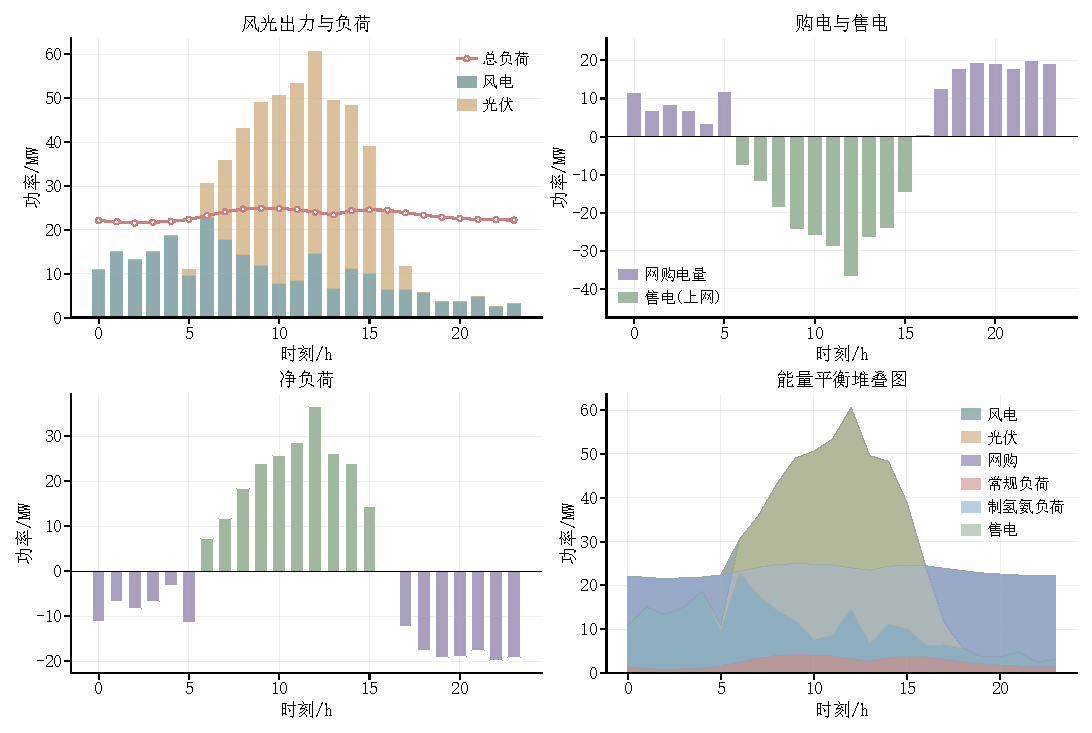
\includegraphics[width=\textwidth]{../figures/q1/fig1_power_balance.pdf}
\caption{园区典型日功率平衡曲线}
\label{fig:q1_balance}
\end{figure}

\cref{fig:q1_balance}从四个维度展示了功率平衡情况：(a)为风电、光伏出力和总负荷的对比，光伏在10:00-14:00出力最大（峰值约46 MW），风电在凌晨和傍晚相对较强（峰值约23 MW）；(b)为购电和售电功率，可见夜间和午间有余电上网，傍晚负荷高峰且光伏归零时需网购电力；(c)为净负荷曲线，正值为余电、负值为缺电，清晰反映了购售电交替规律；(d)为能量平衡堆叠图。

由步骤三和步骤四得到全日能量指标和绿电指标，汇总于\cref{tab:q1_indicators}。

\begin{table}[H]
\centering
\caption{问题一：绿电直连指标与成本}
\label{tab:q1_indicators}
\begin{tabular*}{\textwidth}{@{\extracolsep{\fill}}lcc}
\toprule[1.5pt]
指标 & 计算值 & 要求 \\
\midrule[1pt]
新能源发电量$E_{\mathrm{re}}$ & 603.45 MWh & -- \\
总用电量$E_{\mathrm{total}}$ & 558.72 MWh & -- \\
上网电量$E_{\mathrm{sell}}$ & 216.77 MWh & -- \\
网购电量$E_{\mathrm{buy}}$ & 172.04 MWh & -- \\
自发自用比例$R_{\mathrm{sc}}$ & 28.16\% & $\ge 60\%$ $\times$ \\
总用电绿电比例$R_{\mathrm{g}}$ & 69.21\% & $\ge 30\%$ $\checkmark$ \\
上网电量比例$R_{\mathrm{cur}}$ & 35.92\% & $\le 20\%$ $\times$ \\
吨氨成本$C_{\mathrm{NH_3}}$ & 4322.34 元/吨 & -- \\
\bottomrule[1.5pt]
\end{tabular*}
\end{table}

\cref{tab:q1_indicators}和\cref{fig:q1_radar}使用雷达图直观展示了三个指标与要求值的差距。

\begin{figure}[H]
\centering
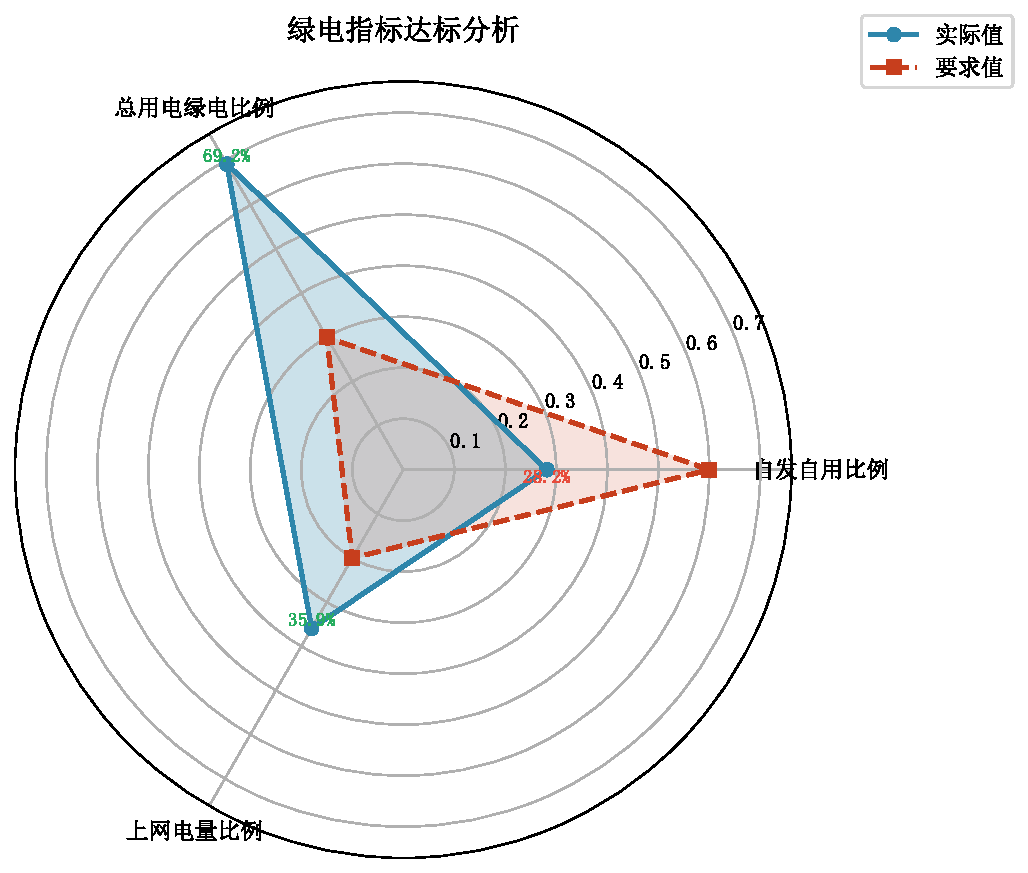
\includegraphics[width=0.55\textwidth]{../figures/q1/fig2_green_indicators_radar.pdf}
\caption{绿电指标达标雷达图}
\label{fig:q1_radar}
\end{figure}

\textbf{原因分析：}三个指标中仅有总用电绿电比例达标（69.21\%），自发自用比例（28.16\%）和上网电量比例（35.92\%）不达标。园区新能源总装机容量104 MW（风电40 MW+光伏64 MW），而制氢氨负荷仅20.75 MW（对应36吨/日产能），总负荷峰值约25 MW。新能源发电能力远超自用需求，大量绿电上网，导致自发自用比例偏低（仅169.91 MWh自用，占发电量的28.16\%）和上网比例偏高（35.92\%）。这一结果表明，36吨/日产能下制氢氨负荷相对于风光装机容量过小，需要通过提升产能或调整可再生能源装机规模来满足绿电直连指标要求\cite{wang2023}。
